\documentclass[11pt]{article}

\newcommand{\cnum}{CS 180}
\newcommand{\ced}{Fall 2019}
\newcommand{\ctitle}[3]{\title{\vspace{-0.5in}\cnum, \ced\\Problem Set #1 #2\\Due #3}}
\usepackage{enumitem}
\newcommand{\solution}[1]{{{\color{black}{} {#1}}}}
\usepackage[usenames,dvipsnames,svgnames,table,hyperref]{xcolor}
\usepackage{graphicx}
\usepackage{amsthm}
\usepackage[tbtags]{amsmath}
\usepackage{amssymb}
\usepackage[hang, small,labelfont=bf,up]{caption} % Custom captions under/above floats in tables or figures
\usepackage{booktabs} % Horizontal rules in tables
\usepackage[mathscr]{euscript} % Euler script font
\usepackage{listings}
\usepackage{tikz}

\definecolor{codegray}{rgb}{0.5,0.5,0.5}
\lstdefinestyle{mystyle}{
	%numberstyle=\tiny\color{codegray},
	numbers=left,
	%numbersep=5pt
}

\lstset{style=mystyle, escapeinside={(/*}{*/)}}

\renewcommand*{\theenumi}{\alph{enumi}}
\renewcommand*\labelenumi{(\theenumi)}
\renewcommand*{\theenumii}{\roman{enumii}}
\renewcommand*\labelenumii{\theenumii.}


\begin{document}
\ctitle{5}{}{November 20, 2019}
\author{Tian Ye \\ \small{UID: 704931660}}
\maketitle
\newpage

\section*{Problem 1}
\fbox{\begin{minipage}{33em}
We will construct $p_x$ and $p_y$, which are points sorted in increasing order of $x$ and $y$, respectively. If we have less than four points, we can call the following algorithm and find the solution in constant time. If there are at least four points, we will divide the problem in half and recursively call it on both halves. Consider the case where there is a shortest distance pair within the left or right half; the recursive call will find it. The case is that the shortest distance is between the left and the right halves. In this case, the algorithm will search for a minimum pair that falls within a distance $d$, or the distance of either individual half.
\end{minipage}}
\begin{lstlisting}
Sort points in x and y dimension in ascending order
Store sorted points into p_x and p_y
Create function dst(a , b) that finds distance

Begin recursive function (p_x, p_y):
	If p has less than four points
		Find and return closest pair via comparison
'	Create two havles of points increasing by x and y
	q_x, q_y, r_x, r_y, divided by a vertical line l
	(q, q') = Function call (q_x, q_y)
	(r, r') = Function call (r_x, r_y)
	Let dist = min(dst(q, q'), dst(r, r'))
	Construct set S containing points within dist of L
	  ordered by increasing y value
	For each point in S
		Find distance to next 15 points in S
		Save minimum pair as s and s'
	If dst(s, s') < dist
		Return (s, s')
	Return minimum pair between dst(q, q') and dst(r, r'))
\end{lstlisting}
\begin{proof}
The algorithm runs in $O(n\log n)$ time complexity as it first sorts the all the points. It then divides the problem into halves, and at each iteration it does at most $O(n)$ work. This yields a net time complexity of $O(n\log n)$.
\end{proof}
\newpage

\section*{Exercise 3 Page 314}
a. \\
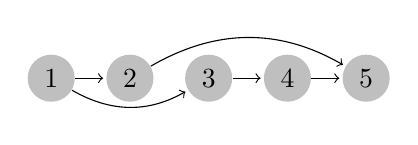
\begin{tikzpicture}[shorten >=1pt,->]
\tikzstyle{vertex}=[circle,fill=black!25,minimum size=17pt,inner sep=0pt]

\node[vertex] (1) {1};
\node[vertex] (2) [right of=1] {2};
\node[vertex] (3) [right of=2] {3};
\node[vertex] (4) [right of=3] {4};
\node[vertex] (5) [right of=4] {5};


\path[every node/.style={font=\sffamily\small}]
(1) edge node [right] {} (2)
(2) edge [bend left] node [right] {} (5)
(1) edge [bend right] node [right] {} (3)
(3) edge node [right] {} (4)
(4) edge node [right] {} (5);

\end{tikzpicture} \\ The given algorithm will find L=3, whereas the correct solution is L=4. \\
b. \\ \\
\fbox{\begin{minipage}{33em}
Each individual subproblem will consider the levels in the vertices, levels being similar to their meaning in a BFS, where each level will contain all $V$ nodes in the graph. There will be at most  $n-1$ levels, any more will imply a cycle. At each level, assuming we have the optimal solution to the previous level, we can use the previous level to solve for the current level's optimal solution. This can be expressed in the following recurrence relation: opt(L, V) = max(opt(L-1, V), max(opt(L-1, V')+1)). V' is some vertex that has an edge to V inside of L-1. To set this up, the base case will have the starting node's opt(0, $v_1$) = 0, while everything else is -1. This leaves two situation in the recurrence relation: either the longest path from the previous level is used, or it is not used when we are calculating the maximal path. In the former, opt(L, V) = opt(L-1, V')+1, as the previous path is taken and incremented by length of 1. In the latter, opt(L, V) = opt(L-1, V), as we are not including that edge from V' to V.
\end{minipage}} \\ \\
opt$(L, V)$ = max(opt$(L-1, V),$ max(opt$(L-1, V')+1))$
\begin{lstlisting}
Initialize array opt[n-1][n-1] = -1
opt[0][1] = 0
For (int L = 1; L < n; L++) 
	For (int i = 0; i < n; i++) 
		For each (v_j that can traverse to v_i) 
			If (opt[L-1][v_j] >= 0) 
				opt[L][v_i] =
				  max(opt[L-1][v_i], 
				  opt[L-1][v_j]+1)
return opt[n-1]
\end{lstlisting}
\begin{proof}
The algorithm runs in $O(n^3)$ time complexity. The first loop iterates through $n-2$ elements, while the second and third loops iterate through $n-1$ elements. Furthermore, the third loop performs constant time operations onto the 2-D array. This results in a time complexity of $O(n^3)$.
\end{proof}
\newpage

\section*{Exercise 5 Page 316}
\fbox{\begin{minipage}{33em}
Defining opt(i) as the highest quality segmentation from the first to the ith character, we will use the following recurrence relation: opt$(i)$ = max\textsubscript{$0 \leq j \leq i$}(quality(substr$(j, i))$ opt$(j-1))$, where we will try all j from 0 to i. To set this up, the base case will have the opt(0) = quality($y_1$), the first character. This leaves us with two situations in the recurrance relation: at position j, being some index from 0 to i, we can either choose to create a segment by cutting at j or we do not. In the former, opt(i) = quality(substr(j, i)) + opt(j - 1), as we will take the optimal for the substring that is up to the position of our cut, and add the quality of the new segment. In the latter case, we choose not to create a segment, and continue on to the next j. This case is trivial; hence we assume at every j we create a segmentation. To find the maximal, we consider the possible segmentation combinations by cutting at each j.
\end{minipage}} \\ \\
opt$(i)$ = max\textsubscript{$0 \leq j \leq i$}(quality(substr$(j, i))$ opt$(j-1))$
\begin{lstlisting}
Create array opt[n] = 0
opt[0] = quality(y_1)
For (int i = 1; i < n; i++)
	For (int j = 0; j<=i; j++)
		opt[i] = max(opt[i], 
		  quality(y_j y_j+1 ... y_i) + opt[j-1])
Return opt[n-1]
\end{lstlisting}
\begin{proof}
The algorithm runs within $O(n^2)$ time complexity, as the outer loop iterates through all n characters, and the inner loop iterates through i characters, being at worst case n. The comparison within the inner loop is constant.
\end{proof}
\newpage

\section*{Exercise 10 Page 321}
a. \\
\begin{table}[!htbp]
\centering
\scalebox{1}{
\begin{tabular}{lccc}
\cmidrule{1-4}
Minute & 1 & 2 & 3 \\
\midrule
A & 10 & 2 & 5 \\
B & 0 & 100 & 10 \\
\bottomrule
\end{tabular}}
\end{table}
The given algorithm finds an answer of 20, while the correct answer is 110. \\
b. \\ \\
\fbox{\begin{minipage}{33em}
We will build the subproblem using the two following recurrence relations: opt(A, i) = max($a_i$ + opt(A, i+1), opt(B, i+1)) ; opt(B, i) = max($b_i$ + opt(B, i+1), opt(A, i+1)). The base case will start at the last minute, in which opt(A, n) = $a_n$ and opt(B, n) = $b_n$. From here, assuming at time i we have built solutions for opt(A, i+1) and opt(B, i+1), we have two options: to keep performing the job on the current machine or to switch machines. In the former, the optimal solution will be to take the weight of the job on the given machine at minute i and add the optimal solution for the job at minute i+1, being $a_i$ + opt(A, i+1) or $b_i$ + opt(B, i+1) on the respective machines. In the latter, the job is moved to another machine. Since switching the job takes time, the optimal solution at minute i is the same as the optimal solution at minute i+1, being opt(B, i+1) and opt(A, i+1) for machines A and B, respectively. We then choose the maximum of the two possibilities at the very end to see if it is more optimal to start on machine A or B.
\end{minipage}} \\ \\
opt(A, i) = max($a_i$ + opt(A, i+1), opt(B, i+1)) \\
opt(B, i) = max($b_i$ + opt(B, i+1), opt(A, i+1))
\begin{lstlisting}
opt_A[n-1], opt_B[n-1]
opt_A[n-1] = a_n
opt_B[n-1] = b_n
For (int i = n-1; i > 0; i++)
	opt_A[i] = max(a_i + opt_A[i+1], opt_B[i+1])
	opt_B[i] = max(b_i + opt_B[i+1], opt_A[i+1])
Return max(opt_A[1], opt_B[1])
\end{lstlisting}
\begin{proof}
The algorithm performs two linear scans on an array of length n, resulting in a time complexity of $O(n)$. The other operations are constant time complexity, yielding an overall time complexity of $O(n)$.
\end{proof}
\newpage

\section*{Exercise 5}
\fbox{\begin{minipage}{33em}
We will use a recurrence relation that considers the solutions to all the subproblems from length 1 to i-1 to solve for the optimal subrod lengths at length i. We will define this as opt(i) = max\textsubscript{$1 \leq j \leq i$}(Price(j) + opt(i-j)) for all j from 1 to i. This yields a base case of opt(0) = 0 and opt(1) = Price(1), since a rod of length 0 will be worth 0 and there is only 1 choice for a rod of length 1. This yields the following possibilities: either we choose to cut the rod at length j or we choose not to. In the former, we are left with a rod of length j and the remainder being a length of i-j. Since we have subproblems that are solved from length 1 to i, this can be represented as opt(i) = Price(j) + opt(i - j). In the latter case, we choose not to cut the rod. This is a trivial case; we always cut the rod to consider all possibilities. This search is exhaustive and will cover all possibilities.
\end{minipage}} \\ \\
opt(i) = max\textsubscript{$1 \leq j \leq i$}(Price(j) + opt(i-j))
\begin{lstlisting}
opt[n] = 0
opt[1] = Price(1)
For (int i = 2; i <= n; i++)
	For (int j = 1; j <= n; j++)
		opt[i] = max(opt[i], Price(j) + opt[i-j])
Return opt[n]
\end{lstlisting}
\begin{proof}
The time complexity is $O(n^2)$, as the outer loop iterates through a maximum of $n$ elements, and the inner loop iterates through another $n$ elements, for a total of $n^2$ elements in the worst cast. The operations within each iteration are constant.\end{proof}
\newpage
\section*{Exercise 6}
\fbox{\begin{minipage}{33em}
We will set $v_i$ as the value of the coin at index i and $v_j$ as the value of the coin at index $j$. We build the following recurrence relation: opt(i, j) = max($v_i$ + min(opt(i+2, j), opt(i+1, j-1)), $v_j$+min(opt(i+1, j-1), opt(i, j-2))). Our base case will be that  opt(n, n)=$v_n$. To prove the correctness of this algorithm, suppose we are considering the optimal solution where we can choose the coin at index i and the coin at index j, where i $\leq$ j. We also assume we have created the optimal choices from 0 to j-1 and i+1 to n. At this point, there are two choices: the player chooses to take the front or the end of the row. In the former, the player chooses the front, denoted by i. We then assume the other player is playing optimally as well, and therefore we take the minimum of what is possible to get after the other player chooses. This is expressed as opt(i, j) = $v_i$ + min(opt(i, j-2), opt(i+1, j-1)). In the latter, the situation is the converse of the former. This is expressed as opt(i, j) = $v_j$ + min(opt(i, j-2), opt(i+1, j-1)). We then combine these two and find the maximum at every iteration to solve for the optimal solution.
\end{minipage}} \\ \\
opt(i, j) = max($v_i$ + min(opt(i+2, j), opt(i+1, j-1)), $v_j$+min(opt(i+1, j-1), opt(i, j-2)))
\begin{lstlisting}
opt[n+1][n+1] = 0
opt[n][n] = v_n
For (int i = n-1; i > 0; i++)
	For (int j = i; j <= n; j++)
		If i == j
			opt[i][j] = v_i
		Else
			opt(i, j) = max(v_i + min(opt(i+2, j), 
			  opt(i+1, j-1)), v_j+min(opt(i+1, j-1),
			  opt(i, j-2)))
Return opt[1][n]
\end{lstlisting}
\begin{proof}
The time complexity is $O(n^2)$, as the outer loop iterates through a maximum of $n$ elements, and the inner loop iterates through another $n$ elements, for a total of $n^2$ elements in the worst cast. The operations within each iteration are constant
\end{proof}
\end{document}